% ENGI 9882 Project Proposal -- IEEE Transactions template (IEEEtran, journal mode)
% Skeleton only: the RED [Write: ...] placeholders mark where YOUR text goes.
% The bullet hints inside them are facts/numbers to cover, not wording to copy.
% Table I and Fig. 1 come from your own runs (qml_feasibility.py output; noise_depth_sweep_FakeManilaV2_5q_scale2.csv).
% FRAMING: an ML project -- weight initialization for quantum neural networks (QNNs), tested on a supervised classifier.
% The Heisenberg reproduction validates the implementation; the noisy hardware simulation tests deployment.
% Limit: max 2 pages (guidance). Delete every placeholder before submitting.
% AUDIENCE (project guidance.pdf): written for the instructor and TAs. Do NOT introduce Adv. ML background
% (gradient descent, Adam, learning rate, initialization schemes, vanishing gradients, variance, seeds...).
% DO introduce the non-Adv. ML topics: the quantum-computing terms listed in Section II, briefly.
% Tip: define each quantum term through an ML analogy the readers already know (angles ~ weights, energy ~ loss).
% Preamble matches IEEE's official Transactions sample (bare_jrnl_new_sample4.tex in TMC_LaTeX_Template.zip),
% plus booktabs (tables), amssymb (math symbols) and xcolor (red placeholders -- remove with \todo when done).
\documentclass[lettersize,journal]{IEEEtran}
\usepackage{amsmath,amsfonts,amssymb}
\usepackage{array}
\usepackage{textcomp}
\usepackage{stfloats}
\usepackage{url}
\usepackage{graphicx}
\usepackage{cite}
\usepackage{booktabs}
\usepackage{xcolor}
\newcommand{\todo}[1]{{\color{red}[Write: #1]}}

\begin{document}

\title{Does Depth-Scaled Gaussian Initialization Make Quantum Neural Networks Trainable? A Reproduction and Its Extension to Classification and Noisy Hardware}
% ^ working title. Shorter alternatives: "Gaussian Initialization for Trainable Quantum Neural Networks";
%   "Escaping Barren Plateaus in Quantum Classifiers: Reproducing and Extending Gaussian Initialization"

\author{
    Kazi Muktadir Ahmed,~\IEEEmembership{Student ID: 202584575}%
}

\markboth{ENGI 9882 \textbar{} Advanced Machine Learning \textbar{} Project Proposal}{}
\maketitle

\begin{abstract}
\todo{About 90 words. (1) Deep quantum neural networks (QNNs) suffer barren plateaus: gradients vanish exponentially with the number of qubits. (2) Zhang et al.\ (NeurIPS 2022) proved that a depth-scaled Gaussian initialization keeps gradients polynomially large, but tested it only on physics and chemistry tasks. (3) This project reproduces their result and tests the initialization on a supervised QNN classifier, both noiseless and in a noisy hardware simulation. (4) Optional headline: at 12 qubits the Gaussian initialization gives a 147$\times$ larger initial gradient than uniform initialization.}
\end{abstract}

\begin{IEEEkeywords}
Quantum machine learning, quantum neural networks, parameter initialization, vanishing gradients, barren plateaus, noisy simulation.
\end{IEEEkeywords}

\section{Problem}
\todo{2--3 sentences, framed as an ML problem (assume ML knowledge; no need to explain vanishing gradients or initialization schemes). Weight initialization decides whether a deep model is trainable (cf.\ Xavier/He for classical networks). For QNNs the failure mode is the barren plateau: with uniformly random initial parameters the gradient variance shrinks exponentially in the number of qubits~\cite{mcclean2018barren}, and QML classifiers inherit it from deep circuits and from the data encoding~\cite{thanasilp2023subtleties}. Number for scale: gradient variance $\sim2^{-N}$, so at $N=15$ a typical gradient $\approx0.0055$ needs $\sim$33{,}000 measurements to resolve.}

\section{Quantum Computing Background}
% Required by the guidance ("introduce non-Adv. ML topics"). One sentence per term; keep the section to ~1 paragraph.
\todo{Introduce only what the proposal uses; cite so readers can follow up (textbook~\cite{nielsen2010quantum}, VQA review~\cite{cerezo2021vqa}):
\begin{itemize}
\item \emph{qubit / state}: $N$ qubits $\to$ a vector of $2^N$ complex amplitudes ($2^{15}=32{,}768$; why 15 qubits fit on a laptop);
\item \emph{gates}: rotations $R_X(\theta)=e^{-i\theta X}$, $R_Y(\theta)=e^{-i\theta Y}$ (Pauli $X,Y,Z$; the angles are the trainable ``weights''), and the entangling CZ gate;
\item \emph{QNN}: data encoding (each input feature sets one rotation angle) $\to$ layers of trainable rotations and CZ gates $\to$ output = expectation value of $Z$ on one qubit, estimated from repeated measurements (``shots''), error $\sim1/\sqrt{\text{shots}}$~\cite{nielsen2010quantum,cerezo2021vqa};
\item \emph{gradients}: the parameter-shift rule, two circuit runs per parameter~\cite{schuld2019gradients};
\item \emph{Hamiltonian / ground energy} (for the reproduction only): minimizing $\langle H\rangle$ finds the lowest energy; each term acts on $S$ qubits (``locality'');
\item \emph{device noise}: gate errors, decoherence ($T_1/T_2$), readout error~\cite{nielsen2010quantum}; IBM ``fake backends'' = noise models calibrated from real chips, run in Qiskit~\cite{javadiabhari2024qiskit}.
\end{itemize}}

\section{Method Under Study}
\todo{Zhang et al.~\cite{zhang2022escaping}, NeurIPS 2022. Cover:
\begin{itemize}
\item the rule $\theta\sim\mathcal{N}(0,\gamma^2)$, $\gamma^2 = 1/(4S(L+2))$: variance shrinks with depth $L$, like Xavier/He shrink it with width; for the classifier ($S=1$, $L=18$) $\gamma^2=1/80$, vs.\ uniform $[0,2\pi]$ variance $3.29$;
\item Theorem~4.1: $\mathbb{E}\|\nabla f\|^2 \ge L/(S^S(L+2)^{S+1})$, i.e.\ polynomial, not exponential, decay;
\item their evidence: a 15-qubit Heisenberg-chain energy minimization and an LiH molecule; the paper names QML classification as a target use (Sec.~3) but does not test it (no need to explain GD/Adam).
\end{itemize}}

\section{Plan}
\todo{Three studies, in priority order:
\begin{itemize}
\item \textbf{S1 Reproduction (validation):} the paper's 15-qubit Heisenberg runs (Gaussian/uniform/zero init $\times$ \{GD, Adam\} $\times$ \{exact, noisy gradients\} $\times$ 5 seeds, 100 iterations) in PennyLane;
\item \textbf{S2 QNN classifier (main ML study):} handwritten digits 3 vs 8 (scikit-learn), PCA to $N$ features, angle encoding, 10 layers, MSE loss on labels $\pm1$; gradient vs.\ qubits $N=4$--14; training at $N=12$ (240 parameters) with Gaussian/uniform/zero init, Adam, 5 seeds; test accuracy and training curves;
\item \textbf{S3 Noisy hardware simulation (deployment):} Qiskit Aer with IBM device noise models (5 and 7 qubits), noiseless vs.\ noisy gradients and training;
\item timeline: results by Nov~20, slides Nov~23, report Dec~7.
\end{itemize}}

\section{Contribution}
\todo{Lead with S2+S3: the first test, to our knowledge, of Zhang et al.'s variance rule on a \emph{deep} QNN classifier where barren plateaus actually occur, and under calibrated device noise. Contrast: a 2026 benchmark of initializations for QNN image classifiers~\cite{rahman2026benchmarking} used two-layer circuits, where it found no severe barren plateaus, and no hardware noise; the original paper models noise only as Gaussian noise on gradients; noise itself causes barren plateaus~\cite{wang2021noise}; the closest noise study uses idealized depolarizing noise and a different small-angle start~\cite{shen2026initialization}. Then: an independent reproduction (S1).}
% References kept in refs.bib for the final report (not cited here): cerezo2021cost, grant2019initialization,
% cerezo2023simulability, derieux2025eqmarl, bergholm2018pennylane.

\section{Preliminary Work}
\todo{2--4 sentences on Table~\ref{tab:qnn} and Fig.~\ref{fig:noise}. Facts: the classifier shows a barren plateau: with uniform init the squared gradient norm falls $65\times$ from 4 to 12 qubits ($3.98\to0.061$), while Gaussian init stays at 1--10 ($147\times$ larger at 12 qubits); a short 8-qubit training run (60 Adam steps) reaches $\approx$0.90 test accuracy for all inits, with lower test MSE for Gaussian (0.27 vs.\ 0.46 uniform), so the training difference must be tested at 10--12 qubits. Reproduction check: a GD run gives $f=-19.2$ (it.~10) and $-22.8$ (it.~100) vs.\ $\approx-19$, $-22.8$ in the paper's Fig.~2(a). Noisy simulation (Fig.~\ref{fig:noise}): Gaussian/uniform gradient ratio grows $4.2\times\to21.8\times$ from 2 to 8 layers.}

\begin{table}[!t]
\caption{QNN classifier (digits 3 vs.\ 8, 10 layers, MSE loss): mean squared gradient norm at initialization over 5 random initializations and 16 training images.}
\label{tab:qnn}
\centering
% Values from qml_feasibility.py, Part 1 (seeded).
\begin{tabular}{@{}rrrrrr@{}}
\toprule
Qubits & Params & Gaussian & Uniform & Zero & G/U \\
\midrule
4  & 80  & 5.68  & 3.98  & 1.03 & 1.4 \\
6  & 120 & 10.19 & 1.35  & 1.06 & 7.5 \\
8  & 160 & 1.27  & 0.45  & 1.00 & 2.8 \\
10 & 200 & 6.68  & 0.12  & 1.07 & 55 \\
12 & 240 & 8.93  & 0.061 & 1.17 & 147 \\
\bottomrule
\end{tabular}
\end{table}

\begin{figure*}[!t]
\centering
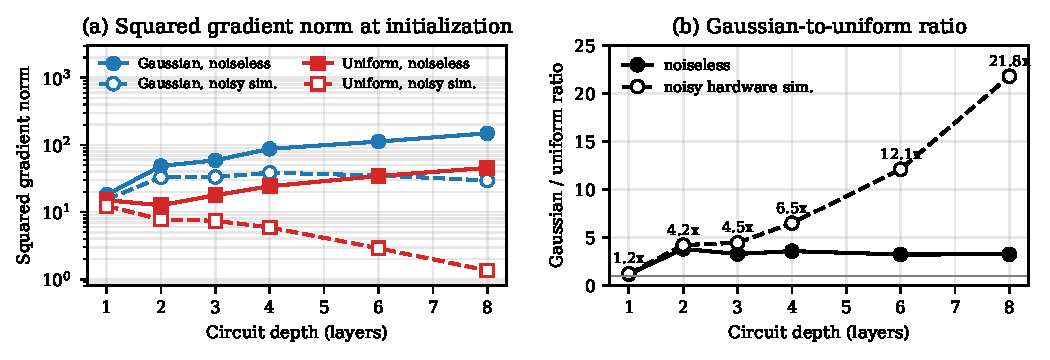
\includegraphics[width=0.85\textwidth]{fig_noise_sweep.pdf}
\caption{Noisy hardware simulation (Qiskit Aer, density matrix, FakeManilaV2 noise model), $N=5$, mean over 8 random draws. (a) Squared gradient norm at initialization vs.\ depth. (b) Gaussian/uniform ratio, noiseless vs.\ noisy (2-qubit gate count after transpilation grows from 17 at 1 block to 154 at 8 blocks).}
\label{fig:noise}
\end{figure*}

\section{Experiment Plan}
% Course outline: hypothesis, proxy statement (metric), protocol, expected results; at most half a page.
\noindent\textbf{Hypothesis.} \todo{e.g.\ on a 12-qubit QNN classifier, where uniform initialization has vanishing gradients, Gaussian initialization reaches a target test accuracy in fewer training steps, and keeps its advantage in the noisy hardware simulation.}

\noindent\textbf{Proxy.} \todo{Statistical: test accuracy, training loss vs.\ steps, steps to reach a target accuracy, $\mathbb{E}\|\nabla f\|^2$ vs.\ qubits. Hardware: wall-clock per training step; circuit evaluations per gradient (parameter shift: $2\times240=480$ per image at 12 qubits); transpiled 2-qubit gate count.}

\noindent\textbf{Protocol.} \todo{S2: $N=12$, 240 parameters, 3 inits $\times$ 5 seeds, Adam (lr 0.01), 100 steps, batch 16, fixed train/test split; $N=4$--14 gradient sweep. S1: the paper's settings. S3: 5 and 7 qubits, noise on/off, 3 seeds.}

\noindent\textbf{Expected results.} \todo{Gaussian $>$ uniform in training speed at $N\ge10$; zero init competitive on the classifier (the encoded input moves it off the flat point) but not on the Heisenberg task; the advantage persists or widens under noise. Negative results are acceptable.}

\bibliographystyle{IEEEtran}
\bibliography{refs}

\end{document}
